%File: supplementary.tex --- Technical Appendix (AAAI-27 supplementary)
\documentclass[letterpaper]{article} % DO NOT CHANGE THIS
\usepackage[submission]{aaai2027}  % DO NOT CHANGE THIS
\usepackage[hyphens]{url}  % DO NOT CHANGE THIS
\usepackage{graphicx} % DO NOT CHANGE THIS
\urlstyle{rm} % DO NOT CHANGE THIS
\def\UrlFont{\rm}  % DO NOT CHANGE THIS
\usepackage{natbib}  % DO NOT CHANGE THIS AND DO NOT ADD ANY OPTIONS TO IT
\usepackage{caption} % DO NOT CHANGE THIS AND DO NOT ADD ANY OPTIONS TO IT
\frenchspacing  % DO NOT CHANGE THIS
\usepackage{booktabs}
\usepackage{amsmath}
\pdfinfo{
/TemplateVersion (2027.1)
}
\setcounter{secnumdepth}{0}

\newcommand{\stage}[1]{\textsc{#1}}

\title{Technical Appendix:\\An Empirical Analysis of Transfer for Dynamic Path Planning}
\author{Anonymous Submission}
\affiliations{}

\begin{document}
\maketitle

\begin{figure*}[t]
\centering

\includegraphics[width=0.98\textwidth]{figures/fig1_program_map.pdf}
\caption{Program map: the three harness ingredients the study isolates---representation and training, planner integration, and formulation/information/supervision---with the stages that intervened at each and their verdicts (orange: failure or negative; blue: positive under the corrected harness; gray: mechanism or null result).}
\label{fig:progmap}
\end{figure*}

\section{A. Protocols by Stage}

All continuous stages share the substrate: a 2-D point robot, maps with procedurally generated obstacles, a probabilistic roadmap (PRM) of $\sim$192 nodes with $k{=}7$ connectivity, and A\textsuperscript{*} evaluated at a per-suite \emph{binding budget} of node expansions calibrated so the algorithmic baseline is neither saturated nor hopeless. Unless noted, training labels are exact graph-Dijkstra costs on the PRM (static) or exact backward space--time Dijkstra values over $(\text{node},t)$ (dynamic). Headline continuous runs are local single-GPU (RTX 5090) validations with one primary training seed unless stated; the discrete program ran on a remote fleet.

\begin{table}[h]
\centering
\footnotesize
\begin{tabular}{@{}lp{5.6cm}@{}}
\toprule
Stage & Protocol essentials \\
\midrule
\stage{C1--C4} & 9 easy suites, $n{=}80$/40 maps, budgets 100--200; pooled bases, TaskLoRA experts, RBF mixtures. \\
\stage{C5} & calibrated hard maze/dense/rooms; 160 train / $\sim$80 eval maps; budgets 128--168; scalar residual target with cap. \\
\stage{C6} & goal-conditioned raster residual field (8 input channels), sampled at PRM nodes; 96/40 maps; budgets 128--168. \\
\stage{C7} & 6 suites (3 held-out families); 96/24 maps per suite; binding budgets 140/24/56; scalar+field $\times$ additive+focal matrix; exact-Dijkstra oracle. \\
\stage{C8} & deterministic moving circular obstacles; space--time PRM; aware ($W{=}8$ future window) vs.\ blind ($W{=}0$) twins; 53 train / 20 eval maps/suite; 1{,}129{,}536 scalar samples. \\
\stage{C9/C9h} & adapt \stage{C7} pooled bases to 3 held-out families; $K\in\{0..32\}$ labeled maps; LoRA(r8, bounded/unbounded), full FT, scratch; \stage{C9h} matches compute (10 epochs, LR $2{\times}10^{-4}$); 30 fixed test maps/target. \\
\stage{C9b} & same protocol on \stage{C8} dynamic sources (aware+blind), 486 adapters, 3 targets, $K\in\{1,4,16\}$. \\
\stage{C10} & 16 rank-8 experts on 2 family axes; zero-label transfer to 3 interior targets; RBF/nearest/uniform weight-merge and prediction-mix composition. \\
\stage{C11} & compositional missions (waypoint sequences; key/door), configs A/B/C, mission length $K\in\{0,2,4,8\}$; 40 train / 25 test maps per cell; 6 learned arms $\times$ 3 seeds (198 checkpoints; 54{,}450 eval rows); exact mission oracle and leg-sum baseline; forced-compute and would-halt probes. \\
\stage{C12} & (A) hidden slow/fast regime dynamics, memory-headroom gate, matched temporal-hierarchy pilot; (B) tied vs.\ untied product-graph refiner, cycles 1--8, configs A/C $\times$ $K\in\{2,8\}$, 3 seeds, 48 checkpoints, two 3{,}200-row test tables. \\
\stage{C13} & current-state heuristic under bounded observation (radius 0.20 local subgraph); behavior-derived fresh-start rollout labels (median of 3); staged falsification ladder (\stage{A}--\stage{L}) then frozen 144-map confirmation (\stage{M}); architecture substitutions (\stage{N}/\stage{O}); persistent-state pilot (\stage{P}). \\
Discrete & 20$\times$20 to 256$\times$256 grids; Manhattan-baseline A\textsuperscript{*}; forecasting (dynamic obstacles), additive residual transfer (22 suites $\times$ 3 budgets $\times$ 100 episodes), pooled multitask bases, learned focal ranking at $w\in\{1.0,1.05,1.1\}$. \\
\bottomrule
\end{tabular}
\caption{Protocol essentials by stage.}
\label{tab:protocols}
\end{table}

\section{B. Full Static and Dynamic Suite Tables}

Tables~\ref{tab:c7} and~\ref{tab:c8} give the complete per-suite \stage{C7} static and \stage{C8} dynamic results summarized in the main paper; Tables~\ref{tab:c8fixed}--\ref{tab:c8seeds} give the fixed-provider primary view and its replications.

\textbf{Multi-seed replication detail (Table~\ref{tab:c8seeds}).} Two full-pipeline retrains (collect + train, seeds 2001/2002) of the aware/blind field U-Net twins were run under a design frozen before training, then evaluated on the same frozen fresh cohort with the canonical binding budgets. Matched-ratio medians across seeds: maze 0.047--0.059, rooms 0.117--0.135, spiral 0.065--0.092 (seed-stable); crossing 0.273--0.434, dense maze 0.216--0.625, large rooms 0.250--0.548 (seed-variable). Preregistered readouts: R1 (success CI excludes zero in $\geq$5/6 suites) 5/6 and 6/6---pass; R2 (deltas within $\pm 0.15$ of canonical in $\geq$5 suites) 5/6 and 6/6---pass; R3 (no suite significantly aware-over-blind) fails as stated for seed 2001 (large rooms $+0.080$ $[+0.020,+0.160]$)---the same suite that is significantly \emph{blind}-better under seed 1234 ($-0.200$ $[-0.320,-0.100]$). Across the 18 seed--suite twin contrasts: 2 significantly aware, 2 significantly blind, 14 null, with the significant cells in different suites for different seeds; the per-suite future-window effects flip sign across seeds and are consistent with training-seed noise. No retraining, reselection, or recalibration occurred in response to any readout.

\textbf{Success as a function of budget (Figure~\ref{fig:budgetcurves}).} A single evaluation pass at $4\times$ the binding budget on the same frozen cohort yields \emph{exact} success-vs-budget curves for every lower budget: the space--time A\textsuperscript{*} expansion order is budget-independent, and a map is solved at budget $B$ iff its recorded solve expansions are $\leq B$, so the curves are derived by thresholding with no re-runs and no interpolation (design frozen before launch). As a determinism cross-check, thresholding at the binding budget reproduces every fresh-cohort success value exactly (all suites, all providers). The headline result is not an artifact of the calibrated operating point: Euclidean search needs 1.7--2.8$\times$ the binding budget to reach the fixed blind provider's binding-budget success (crossing 2.49$\times$, maze 2.29$\times$, dense maze 1.95$\times$, rooms 1.73$\times$, large rooms 1.94$\times$, spiral 2.80$\times$), and by $4\times$ the binding budget every provider converges to the same feasibility ceiling (0.94--1.00; on dense maze the 0.94 ceiling binds even the oracle, reflecting maps unsolvable within the time horizon).

\begin{figure}[t]
\centering
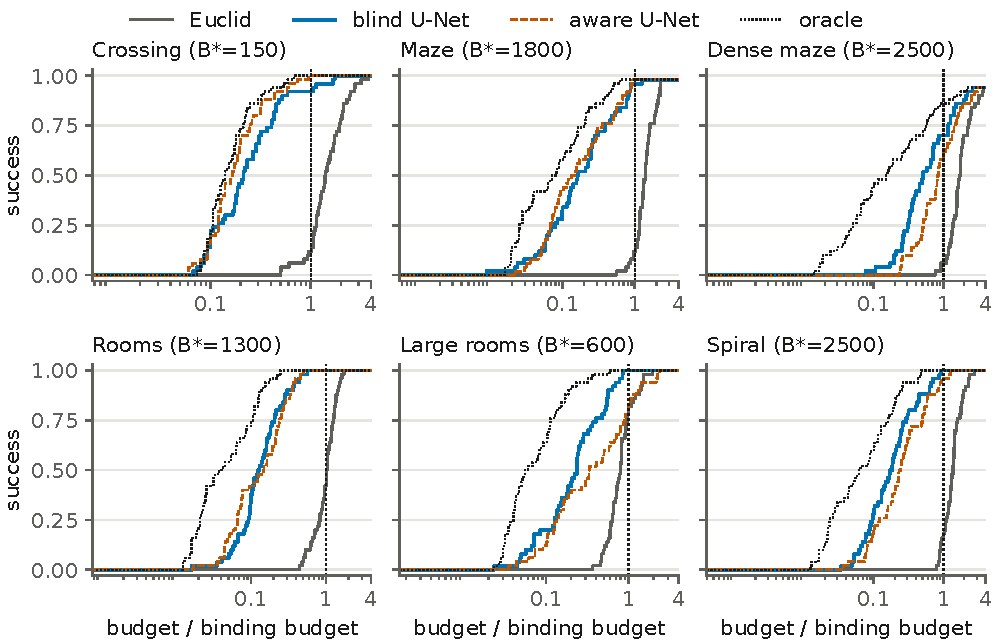
\includegraphics[width=\columnwidth]{figures/fig_budget_curves.pdf}
\caption{Success-vs-budget step curves per dynamic suite (fresh 50-map cohort), derived exactly from one $4\times$-binding evaluation pass. Budgets are normalized by the binding budget $B^{*}$ (dashed vertical line). The learned providers reach high success at 0.05--0.3$\times$ $B^{*}$; Euclid requires 1.7--2.8$\times$ $B^{*}$ to match the blind provider's binding-budget success.}
\label{fig:budgetcurves}
\end{figure}

\begin{table}[h]
\centering
\footnotesize
\setlength{\tabcolsep}{3pt}
\begin{tabular}{@{}lccc@{}}
\toprule
Suite & Euclid succ. & Field-HRM succ. & Ratio [95\% CI] \\
\midrule
Maze & 0.583 & 1.000 & 0.521 [0.450, 0.627] \\
Maze-dense & 0.250 & 0.958 & 0.804 [0.707, 0.829] \\
Rooms & 0.375 & 0.958 & 0.829 [0.775, 0.885] \\
Spiral & 0.250 & 0.917 & 0.850 [0.742, 0.919] \\
Bugtrap & 0.458 & 0.750 & 0.714 [0.533, 0.800] \\
Rooms-large & 0.417 & 0.750 & 0.839 [0.646, 1.222] \\
\bottomrule
\end{tabular}
\caption{\stage{C7} static suites at binding budgets: success and matched-solved median expansion ratio (field HRM vs.\ Euclid). Success gains are BH-significant in 4/6 suites (maze, dense, rooms, spiral); bugtrap and rooms-large reach corrected significance only for other learned arms. Scalar-HRM ratios span 0.427--0.822. Matched $n$ ranges 6--14.}
\label{tab:c7}
\end{table}

\begin{table}[h]
\centering
\scriptsize
\setlength{\tabcolsep}{3pt}
\begin{tabular}{@{}lcccc@{}}
\toprule
Suite & Euclid succ. & Blind U-Net succ. & Ratio [95\% CI] & $n$ \\
\midrule
Crossing & 0.30 & 0.95 & 0.191 [0.166, 0.878] & 6 \\
Maze & 0.30 & 1.00 & 0.093 [0.057, 0.137] & 6 \\
Dense maze & 0.05 & 0.75 & 0.246 (descriptive) & 1 \\
Rooms & 0.30 & 1.00 & 0.099 [0.050, 0.214] & 6 \\
Large rooms & 0.75 & 0.95 & 0.228 [0.185, 0.418] & 15 \\
Spiral & 0.20 & 0.95 & 0.087 [0.061, 0.287] & 4 \\
\bottomrule
\end{tabular}
\caption{\stage{C8} fixed-provider result on the \emph{original} 20-map cohort (field U-Net blind; no future-motion input; additive mode; binding budgets; map-level bootstraps). Success deltas are $+0.20$ to $+0.75$ with all six paired CIs excluding zero.}
\label{tab:c8fixed}
\end{table}

\begin{table}[h]
\centering
\scriptsize
\setlength{\tabcolsep}{3pt}
\begin{tabular}{@{}lcccc@{}}
\toprule
Suite & Euclid succ. & Blind U-Net succ. & Ratio [95\% CI] & $n$ \\
\midrule
Crossing & 0.12 & 0.92 & 0.273 [0.109, 0.516] & 6 \\
Maze & 0.12 & 0.96 & 0.047 [0.021, 0.153] & 6 \\
Dense maze & 0.06 & 0.70 & 0.216 [0.100, 0.281] & 3 \\
Rooms & 0.42 & 1.00 & 0.121 [0.106, 0.172] & 21 \\
Large rooms & 0.82 & 1.00 & 0.250 [0.188, 0.306] & 41 \\
Spiral & 0.16 & 1.00 & 0.092 [0.065, 0.146] & 8 \\
\bottomrule
\end{tabular}
\caption{\stage{C8} fixed-provider \emph{replication} on the fresh 50-map-per-suite cohort (generation seed 999999, frozen before any result was observed; map-disjoint from the original cohort by the evaluation seed formula's within-suite offset bound). Success deltas are $+0.18$ to $+0.84$ with all six paired CIs excluding zero. Map-paired aware$-$blind success deltas on this cohort: crossing $+0.080$ $[+0.020,+0.160]$, maze $+0.020$ $[0.000,+0.060]$, dense maze $-0.120$ $[-0.220,-0.040]$, rooms $0.000$, large rooms $-0.200$ $[-0.320,-0.100]$, spiral $-0.040$ $[-0.100,0.000]$: one suite significantly favors the aware twin, two the blind twin, three neither.}
\label{tab:c8fresh}
\end{table}

\begin{table}[t]
\centering
\scriptsize
\setlength{\tabcolsep}{2.6pt}
\begin{tabular}{@{}lccc@{}}
\toprule
Suite & Seed 1234 & Seed 2001 & Seed 2002 \\
\midrule
Crossing & $+0.80$ [0.68, 0.90] & $+0.86$ [0.74, 0.96] & $+0.88$ [0.78, 0.96] \\
Maze & $+0.84$ [0.74, 0.94] & $+0.86$ [0.76, 0.96] & $+0.84$ [0.74, 0.94] \\
Dense maze & $+0.64$ [0.50, 0.78] & $+0.46$ [0.32, 0.60] & $+0.56$ [0.42, 0.70] \\
Rooms & $+0.58$ [0.44, 0.72] & $+0.58$ [0.44, 0.72] & $+0.58$ [0.44, 0.72] \\
Large rooms & $+0.18$ [0.08, 0.30] & $+0.10$ [$-$0.02, 0.22] & $+0.16$ [0.06, 0.26] \\
Spiral & $+0.84$ [0.74, 0.94] & $+0.84$ [0.74, 0.94] & $+0.84$ [0.74, 0.94] \\
\bottomrule
\end{tabular}
\caption{\stage{C8} preregistered multi-seed replication: paired success deltas (blind U-Net $-$ Euclid, map-level 95\% CIs) for three independent training seeds on the same frozen fresh cohort. 17 of 18 CIs exclude zero; the single crossing interval is seed 2001's near-ceiling large-rooms cell (Euclid 0.82).}
\label{tab:c8seeds}
\end{table}

\begin{table}[h]
\centering
\scriptsize
\setlength{\tabcolsep}{3pt}
\begin{tabular}{@{}lccc@{}}
\toprule
Suite (arm) & Succ.\ E$\to$L & Ratio [95\% CI] & Matched $n$ \\
\midrule
Crossing (U-Net) & 0.30$\to$1.00 & 0.258 [0.132, 0.769] & 6 \\
Maze (U-Net) & 0.30$\to$1.00 & 0.064 [0.046, 0.088] & 6 \\
Maze-dense (U-Net) & 0.05$\to$0.75 & 0.278 (no CI) & 1 \\
Rooms (U-Net) & 0.30$\to$1.00 & 0.096 [0.038, 0.191] & 6 \\
Rooms-large (U-Net) & 0.75$\to$0.90 & 0.380 [0.132, 0.591] & 14 \\
Spiral (field HRM) & 0.20$\to$0.90 & 0.046 [0.038, 0.073] & 4 \\
\bottomrule
\end{tabular}
\caption{\stage{C8} \emph{secondary} view: per-suite strongest arms (explicitly post-hoc selection). Corrected success evidence holds on five suites; rooms-large is supported mainly by expansion evidence. Dense-maze has matched $n{=}1$ and supports no expansion inference. Blind arms are the per-suite best in five of six suites.}
\label{tab:c8}
\end{table}

\section{C. Transfer and Composition Details}

Representative \stage{C9} HRM curves (ratio at success): maze-dense LoRA $0.650$ (1.00) at $K{=}1$ to $0.730$ (0.97) at $K{=}16$; maze-dense full FT $0.744$ (0.76) to $0.571$ (0.99) at $K{=}16$ and $0.552$ at $K{=}32$; scratch $1.008$ (0.37) to $0.808$ (0.80); rooms-large full FT $1.128$ (0.37) at $K{=}1$ to $0.500$ (0.92) at $K{=}8$; bugtrap LoRA degrades from $\approx$0.696 (0.83) to $0.950$ (0.48) at $K{=}32$---LoRA is usually but not universally base-preserving. \stage{C9h} (matched compute): bounded-minus-unbounded LoRA median ratio delta $0.000\pm0.008$ across 27 cells (22/27 exactly zero; max $|\Delta|$ 0.028); rooms-large field U-Net full FT reaches $0.404$ at 0.97 success from $0.982$ zero-shot while conv-LoRA stays at $0.992$--$1.002$. \stage{C9b} (dynamics): maze-dense aware U-Net zero-shot $0.145$ (0.60), LoRA $K{=}16$ $0.059$ (0.97), full FT $K{=}1$ $0.112$ (0.70); aware-minus-blind success deltas at full-FT $K{=}16$ are $0.00$ or $-0.05$ in all nine cells. \stage{C10}: RBF-merge minus zero-shot expansion-ratio deltas by target/backbone: $-0.022$, $-0.012$, $-0.024$, $+0.082$, $+0.012$, $+0.116$; weight-space vs.\ prediction-space deltas lie within $[-0.012, +0.007]$; own-axis RBF mass 0.986--0.998.

\section{D. \stage{C11} Gates, Collapse Forensics, and Scale}

\begin{table}[h]
\centering
\footnotesize
\begin{tabular}{@{}lp{5.2cm}@{}}
\toprule
Gate & Verdict \\
\midrule
K=0 continuity & FAIL, diagnosed as false premise: \stage{C7} had no MLP arm and did not give every architecture the \stage{C11} input; real shallow separation plus collapsed recurrent cells violate the all-tie assumption. Measurement layer verified. \\
G1 dose--response & Negative: no structured arm beats MLP at $\geq$2 mission depths with non-decreasing gap. \\
G2a forced compute & Negative: HRM-v2 $k{=}1/2/4/8$ expansion and MAE curves flat in every $K{=}8$ config. \\
G2b learned halting & Negative, inverted: pooled Spearman $\rho{=}-0.407$, permutation $p{\approx}5{\times}10^{-4}$, $n{=}675$; mean would-halt steps 6.79/7.01/5.30 at $K{=}2/4/8$. \\
G3 closure & Neither preregistered branch: global-input arms separate at shallow $K$ (U-Net/GNN vs.\ MLP ratios $\approx$0.67--0.87; state MAE 0.151/0.171 vs.\ 0.251 at A/$K{=}0$), but no arm converts depth into growing advantage. \\
\bottomrule
\end{tabular}
\caption{\stage{C11} preregistered gates.}
\label{tab:c11gates}
\end{table}

\textbf{Collapse forensics.} Five of 33 recurrent/ACT arm-cells show constant-prediction or partial seed collapse (HRM-trace A8/C8, ON-LSTM B0, HRM-v2 B0, two ON-LSTM A8 seeds), with a reproducible loss signature at the normalization cap. The largest recurrent deficits (HRM-trace ratios 1.526 at A8, 1.600 at C8) are collapse measurements, not expressiveness estimates. Removing $K{=}0$ padding \emph{worsens} recurrent predictions: models used pad steps as extra recurrent compute.

\textbf{Scaled addendum.} A 12-run \texttt{unet\_film\_big} vs.\ \texttt{hrm\_trace\_big} comparison (complete; 2{,}700 eval rows) preserves the ordering: completion 0.804 vs.\ 0.736 at $K{=}2$ and 0.413 vs.\ 0.307 at $K{=}8$; mean state MAE 0.395 vs.\ 0.447 ($K{=}2$) and 0.906 vs.\ 1.855 ($K{=}8$). At $K{=}8$ the scaled HRM exactly matches the leg-sum baseline's completion and mean expansions (0.307; 701.34)---persistent collapse, not recovered hierarchy.

\section{E. \stage{C12} Detail}

\stage{C12-A} (memory headroom, then learned pilot): constructed decision-relevant aliasing at 71.3\% of paired decisions; privileged mode/history diagnostic $+0.467$ completion and $-65.1$\% collision-adjusted regret (map-bootstrap 95\% CI 63.0--66.9\%); oracle completion 0.975. The one-seed matched temporal-hierarchy pilot fails G1 (forecast), G2 (planning), and G3 (persistent carry); overall \emph{strong negative}. \stage{C12-B} (tied refiner): cycle-1$\to$8 normalized burden improves monotonically in every cell (A/$K2$ 0.859$\to$0.815; A/$K8$ 0.624$\to$0.576; C/$K2$ 0.867$\to$0.777; C/$K8$ 0.576$\to$0.517; all cycle-1/8 map-bootstrap intervals separate), but the $K8{-}K2$ gain is $+0.0038$ (CI $[-0.0199, 0.0281]$) on A and $-0.0305$ ($[-0.0726, 0.0096]$) on C---no dose--response. Tied beats shallow and untied on C/$K8$ (deltas 0.0177/0.0076, BH $q{=}6.7{\times}10^{-5}$) but loses to untied on A/$K8$ ($q{=}0.0168$). Bellman residual \emph{worsens} over cycles in every cell while burden improves; solved cycle-8 paths average 1.4--2.2\% above oracle cost. $K{=}16$ was dropped before training by a construction gate (only 2/300 and 1/300 valid missions).

\section{F. C13: Mechanism Ladder and Frozen Confirmation}

\textbf{Claim supported.} A provider restricted to bounded local observations (radius-0.20 subgraph on a known roadmap; behavior-derived labels; no shortest-path supervision) can, with one inference-time local Bellman backup, beat every fixed complete-map \stage{C7} provider in pooled expansions at matched empirical path quality on a frozen, disjoint cohort.

\textbf{Ladder.} Each rung changes one factor; deltas are paired expansions versus the matched comparator (rungs C--G versus matched focal search at $w{=}1.10$, including oracle providers on six development maps; rungs I--M versus the complete-map field HRM, live on all six suites).

\begin{table}[h]
\centering
\scriptsize
\setlength{\tabcolsep}{3pt}
\begin{tabular}{@{}llr@{}}
\toprule
Rung & Factor changed & $\Delta$ exp.\ [95\% CI] \\
\midrule
C & fresh certifier (oracle rank) & $+11.50$ (0/6 wins) \\
D & shared-queue certifier (oracle rank) & $-6.83$ (6/6 wins) \\
E & exact rollout rank & $+1.33$ (2/6) \\
F & monotone recalibration & $+1.33$ \\
G & analytic local escape & $+6.83$ (0/6) \\
I & one-family model, live six suites & $+15.36$ $[+12.02,+18.64]$ \\
J & suite-balanced training, static insert & $+16.17$ $[+9.67,+22.67]$ \\
K & + one local Bellman backup & $-1.21$ $[-8.04,+5.46]$ \\
L & + scale $\alpha{=}1.50$ (48 fresh maps) & $-13.04$ $[-18.67,-7.65]$ \\
M & frozen 144-map confirmation & $-12.96$ $[-16.30,-9.74]$ \\
\bottomrule
\end{tabular}
\caption{The \stage{C13} falsification ladder. Target repairs (E, F), analytic constructions (G), and distribution repairs (I, J) fail; the integration repair (K) plus scale calibration (L) flip the sign, and the frozen confirmation (M) reproduces it.}
\label{tab:c13ladder}
\end{table}

\textbf{Frozen confirmation, per suite.} 144 maps (24 per family; seeds disjoint from every prior cohort; feature caches hash-verified against live regeneration; model, radius 0.20, $\alpha{=}1.50$, integration, and analysis frozen before generation).

\begin{table}[h]
\centering
\scriptsize
\setlength{\tabcolsep}{2.5pt}
\begin{tabular}{@{}lrrrlr@{}}
\toprule
Suite & Local & Field HRM & $\Delta$ & 95\% CI & W/T/L \\
\midrule
Maze & 47.63 & 84.38 & $-36.75$ & $[-45.58,-27.83]$ & 24/0/0 \\
Dense maze & 95.38 & 104.50 & $-9.13$ & $[-15.21,-3.13]$ & 18/1/5 \\
Rooms & 98.04 & 106.17 & $-8.13$ & $[-14.33,-1.71]$ & 16/0/8 \\
Spiral & 120.25 & 121.33 & $-1.08$ & $[-5.88,+4.21]$ & 14/1/9 \\
Bugtrap & 14.96 & 24.29 & $-9.33$ & $[-17.79,-2.92]$ & 18/1/5 \\
Large rooms & 33.58 & 46.92 & $-13.33$ & $[-18.92,-7.50]$ & 19/0/5 \\
\midrule
Pooled & 68.31 & 81.26 & $-12.96$ & $[-16.30,-9.74]$ & 109/3/32 \\
\bottomrule
\end{tabular}
\caption{\stage{C13-M} per-suite paired expansion deltas versus the complete-map field-HRM comparator. Every suite mean is negative; the spiral interval crosses zero, and the preregistered gate is pooled with a suite-breadth condition (at least four negative suite means), which passes. The local provider also beats every other fixed \stage{C7} learned provider in pooled expansions on this cohort.}
\label{tab:c13msuite}
\end{table}

\textbf{Scale calibration.} On the disjoint 48-map calibration block, $\alpha\in\{1.00,1.25,1.50,2.00\}$ gives deltas $-3.79$ $[-9.40,+1.73]$, $-9.77$ $[-15.38,-4.42]$, $-13.04$ $[-18.67,-7.65]$, and $-16.94$ $[-22.56,-11.54]$, with 4/4/6/6 negative suite means and mean/max cost ratios rising from 1.022/1.241 to 1.052/1.366; $\alpha{=}1.50$ was frozen as the largest scale whose suite breadth was complete before the absolute-ceiling verdict, and every arm formally fails the preregistered absolute 1.10 maximum-cost ceiling---the confirmation gate is therefore comparator-relative (mean within $+0.005$, max within $+0.02$ of field HRM), which passes with margins to spare (1.0235/1.1624 vs.\ 1.0311/1.3346).

\textbf{Operating points and timing.} The direct $\alpha{=}1.50$ arm is the matched-quality expansion result and carries no formal bound. The separate certified operating point runs the learned rank inside a $w{=}1.10$ focal band with a shared-queue consistent-bound incumbent proof and passes all 144 bound and certificate checks. Per-map wall time decomposes as feature construction 5.138\,s (prototype Python builder), model inference 0.0008\,s, local backup 0.0097\,s, and search 0.0002\,s, versus 0.371\,s complete-map field-HRM inference: the result is search effort and path quality, not latency.

\textbf{Architecture substitutions under the identical method} (\stage{C13-N/O/P}) are summarized in the main paper; their raw artifacts (development grids, verdicts, integrity manifests) ship in the artifact package.

\section{G. Discrete Program Detail}

The discrete program is substantially larger than the canonical subset reported here: fifteen experiment families across eleven surveyed cloud volumes (13{,}671 parsed result files) and roughly thirty experiment scripts, including a ten-run early scaling lineage of obstacle-trajectory forecasters, diffusion path-generator baselines, a superseded harder-calibration predecessor of the structured protocol below, partial precursors of the controlled transfer run, an empty-model baseline-rerun control (static A\textsuperscript{*} re-verified through the learned-model code path), and a budget-invariance analysis establishing that raising search budgets adds work without rescuing success on the hard families. The paragraphs below report the completed canonical results; the full inventory ships with the released artifacts.

\textbf{Forecasting.} Matched 100-episode protocol: HRM-3M/10M 71/100 vs.\ LSTM 67--69/100 (no uncertainty reported; two-episode matched gap). Structured Preset~M+ (four 100-episode suites): ON-LSTM-10M 0.3875 mean success vs.\ HRM-10M 0.2650 and HRM-3M 0.200; ON-LSTM-3M also has the lowest rollout MSE (0.1257/1.1269 one-/five-step vs.\ 0.3973/2.6438 for HRM-3M).

\textbf{Additive transfer (clean v3, 22 suites $\times$ 3 budgets).} Manhattan 0.590 success / 126{,}707 mean expansions; HRM full-FT 0.585 / 128{,}013; ON-LSTM full-FT 0.564 / 127{,}228; HRM LoRA 0.554 / 140{,}852; ON-LSTM LoRA 0.514 / 145{,}282. Every learned arm $\leq$ matched baseline.

\textbf{Pooled multitask.} HRM pooled base 0.612 success ($+2.11$pp) / 122{,}184 expansions vs.\ Manhattan 0.591 / 126{,}630---the strongest completed discrete additive positive; only 1 of several specialists beats its matched four-suite baseline ($+2.0$pp; others $-0.42$ to $-20.25$pp).

\textbf{Focal ranking (local pilot, 3--8 seeds).} Magnitude is scale-flat despite near-perfect ordering (correlation 0.987--0.994; predicted/true mean 0.73/0.42/0.27/0.19 at 64/128/192/256). At $w{=}1.0$: HRM A128-static ratio 0.85 with success 0.62$\to$0.75; A192 0.94 (0.75$\to$0.75); A128-dynamic 0.93 (0.62$\to$0.62); ON-LSTM A128/A192 0.85 (0.75$\to$0.75). At $w{=}1.05$, A128-dynamic improves further but A192 success regresses 0.75$\to$0.62; $w{=}1.0$ is the evidence-safe operating point. Experts exactly match pooled bases in tested cells.

\section{H. Validity Forensics}

\textbf{The frozen-halt artifact.} A 27.27M-parameter direct maze solver reported 96.64\% token accuracy, 25.40\% exact accuracy, and ``74.60\% halt accuracy'' with 16 average adaptive-computation steps. Audit: $74.60 = 100 - 25.40$ exactly---the halt logit was frozen negative (a constant-false classifier) because the training loop omitted the halt loss and back-propagated only the final segment. After repairing the loss path (verified live: halt loss 0.14$\to$0.06, token accuracy 90--95\%), exact accuracy remained 0.000 at the chosen stop point; the repaired run demonstrates mechanism liveness, not task convergence. Bit-exact forward parity with the reference implementation was separately established. We recommend the $100{-}x$ pattern as a standard red flag for adaptive-computation metrics.

\textbf{The cap-collapse signature.} \stage{C5}'s scalar HRM collapse sits at a loss value pinned by the residual cap (2.612 in that setup, with constant predictions at the cap). The same class of signature reappears in \stage{C11}: collapsed cells share an \emph{identical} final loss (1.1397, exactly the constant-cap loss under that normalization), enabling automatic collapse detection instead of misreading collapsed cells as capacity evidence.

\textbf{Pad steps as compute.} In \stage{C11}, removing $K{=}0$ padding tokens \emph{degraded} recurrent predictions---models had co-opted padding as additional recurrent iterations. Sequence-model comparisons that alter padding alter compute.

\section{I. Statistics}

Success is compared with paired McNemar tests, BH-corrected within stage families. Expansion effort is compared only on matched solved maps via median ratios with bootstrap percentile CIs (10k--20k resamples); from \stage{C12} onward, bootstraps are map-clustered by design. \stage{C9}--\stage{C11} originally pooled repeated evaluations of fixed test maps across adaptation/model seeds; Section~J reports the map-clustered reanalysis of every quantity the main paper quotes from those stages; the fixed-provider dynamic reanalysis of Table~\ref{tab:c8fixed} uses the same map-level grain. Matched-solved ratios condition on joint success and can favor arms that solve only easier maps; we therefore always report success and ratios separately and never combine them into a single score. Negative results are failures to observe an effect under the tested protocol, not equivalence claims; no equivalence tests were run.

\section{J. Map-Clustered Reanalysis}

Units are test maps; adaptation/model seeds are averaged within maps before inference; success deltas use 10{,}000-resample map bootstraps; expansion ratios are medians of per-map ratios over matched maps at the binding budget in additive mode; the \stage{C11} halting test aggregates model seeds within maps and permutes mission length within config (maps are independent across $K$ cells; 20{,}000 stratified permutations). Estimator conventions differ slightly from the published record-level curves, so point values differ modestly; the question is verdict-level agreement. A methodological caution surfaced during this work: a first pass that accidentally pooled additive and focal evaluation modes attenuated the apparent \stage{C9} transfer effects by roughly half---mode/aggregation mixing alone can manufacture or destroy an effect of the size under study.

\textbf{\stage{C11} halting.} Record level reproduces the published value ($\rho{=}-0.4066$, $n{=}675$); map level strengthens it ($\rho{=}-0.5778$, $n{=}225$, stratified permutation $p{=}5{\times}10^{-5}$). Map-level means 6.78/7.01/5.30 at $K{=}2/4/8$.

\textbf{\stage{C11} vs-MLP ratios.} Map-clustered ratio-of-means CIs exclude parity at $K\in\{0,2\}$ in config A for both U-Net (0.734/0.846) and GNN (0.822/0.923), and in config B at $K{=}0$ (0.904/0.818) plus B/$K{=}2$ for the GNN (0.805); config C never separates; every $K\in\{4,8\}$ cell includes parity.

\begin{table}[h]
\centering
\scriptsize
\setlength{\tabcolsep}{2.5pt}
\begin{tabular}{@{}lll@{}}
\toprule
Cell (HRM) & $\Delta$success [CI] & map ratio [CI] \\
\midrule
dense LoRA $K{=}1$ & $+0.467$ $[+0.300,+0.633]$ & 0.686 $[0.590,0.774]$ \\
dense LoRA $K{=}16$ & $+0.433$ $[+0.267,+0.600]$ & 0.786 $[0.694,0.891]$ \\
dense full $K{=}1$ & $+0.227$ $[+0.080,+0.380]$ & 0.789 $[0.751,0.836]$ \\
dense full $K{=}16$ & $+0.460$ $[+0.287,+0.633]$ & \textbf{0.610} $[0.549,0.670]$ \\
dense scratch $K{=}1$ & $-0.167$ $[-0.300,-0.047]$ & 1.035 $[1.029,1.039]$ \\
rl.\ full $K{=}1$ & $-0.167$ $[-0.340,+0.013]$ & 1.293 $[1.170,1.503]$ \\
rl.\ full $K{=}8$ & $+0.387$ $[+0.227,+0.547]$ & 0.590 $[0.498,0.712]$ \\
bug.\ LoRA $K{=}32$ & $-0.320$ $[-0.507,-0.133]$ & 1.153 $[1.012,1.523]$ \\
\bottomrule
\end{tabular}
\caption{Map-clustered \stage{C9} key cells (binding budgets, additive mode; dense = maze-dense, rl.\ = rooms-large, bug.\ = bugtrap). The $K{=}16$ full-FT/LoRA CIs are disjoint (the crossover), the rooms-large $K{=}1$ catastrophe excludes parity, and the bugtrap LoRA degradation is significant in both metrics.}
\label{tab:wcr-c9}
\end{table}

\textbf{\stage{C9h} bound-vs-capacity.} 27 cells: median bounded-minus-unbounded map-level ratio delta $+0.0000$; 15/27 exactly zero; sd 0.0077; max $|\Delta|$ 0.0370---the capacity attribution stands.

\textbf{\stage{C9b} aware$-$blind (full FT, $K{=}16$).} Eight of nine point deltas are zero or negative; the single positive ($+0.017$ $[0.000,+0.050]$) does not exclude zero; no cell shows a significant aware advantage.

\textbf{\stage{C10} composition.} Map-paired deltas vs.\ zero-shot: four cells $\approx$0 with CIs crossing zero; the two ON-LSTM rooms cells are significantly \emph{worse} ($+0.089$ $[+0.061,+0.121]$ and $+0.098$ $[+0.076,+0.123]$), matching the published point deltas and upgrading the null to ``never better, sometimes significantly worse.''

No preregistered verdict flips under any of these recomputations.

\section{K. Reproducibility and Artifact Inventory}

From \stage{C7} onward every stage freezes a written design (gates, budgets, analysis grain) before execution; artifacts (checkpoints, feature caches, cohort manifests, raw rows, verdicts, reports) are hash-bound in integrity manifests; confirmation cohorts are generated only after freezing model, integration, and evaluation code; failed development gates block confirmation rather than triggering retuning. Duplicate-evaluation determinism is enforced where preregistered (byte-identical traces; identical decision rows). The final-stage pilot on persistent planning-time state ran under a fully test-verified harness (158 focused-plus-neighboring tests; hardware preflight). Its first staged execution ended at a preregistered execution-integrity hard stop---the harness's independent reanalysis disagreed with the primary comparison computation, voiding all mechanism fields. After repair of the named defect only, a fresh-fingerprint rerun passed every integrity primitive, including independent reconstruction of the comparison evidence from promoted raw artifacts, and returned the valid negative reported in the main paper: persistent carry loses to the same-checkpoint reset twin on map-macro frontier ranking (MRR delta $-0.029$, 95\% CI $[-0.060,-0.003]$), and no self-bootstrap or confirmation was run. We note the initial stop as the integrity machinery functioning as designed.

The anonymized artifact archive submitted with this paper contains: (i) the analysis scripts that regenerate every main-paper figure and quoted map-level statistic from raw rows (the fixed-provider dynamic reanalysis, the map-clustered reanalysis, and all figure generators); (ii) the raw paired evaluation rows behind every quoted quantity (\stage{C7}/\stage{C8} evaluation tables, including the fresh-cohort and three-seed replication rows, \stage{C9}/\stage{C9h}/\stage{C9b}/\stage{C10} evaluation tables, \stage{C11} evaluation and halting tables, and \stage{C13} development and confirmation rows); (iii) map/cohort manifests, seed lists, frozen configurations, and the integrity manifests for the frozen confirmations; (iv) the preregistration design documents from \stage{C7} onward; and (v) a top-level README with reproduction commands and expected outputs. Checkpoints are included where size permits; otherwise exact training commands and configurations are provided.

\section{L. C14: Label-Count $\times$ World-Diversity Factorial}

A preregistered factorial (design and pre-execution amendment in the artifact package) tests whether the LoRA/full-fine-tuning contrast is governed by the number of supervised search states $N$, independent of domain and map count. Factors: $N \in \{256, 1024, 4096, 16384, 65536\}$ exact-count state samples $\times$ two diversity levels at fixed $N$ (concentrated: the minimal world count $w_{\min}(N)$; distributed: $8 \times w_{\min}(N)$ worlds) $\times$ two domains (static \stage{C9} substrate and dynamic \stage{C9b} substrate, maze-dense target, frozen sources) $\times$ \{unbounded rank-8 LoRA, full fine-tuning, scratch\} $\times$ 3 seeds --- 180 adaptations, every cell at an identical 2{,}560 optimizer steps, evaluated on the frozen \stage{C9}/\stage{C9b} test cohorts at binding budgets. The measured $w_{\min}$ spans quantify the domains' supervision densities: reaching $N{=}65{,}536$ takes 356 static worlds but 4 dynamic worlds ($\sim$185 vs.\ $\sim$18{,}900 usable states per world).

\textbf{Preregistered verdict: H-C14 rejected as stated.} On matched-solved expansion ratios the hypothesized crossover point is degenerate: full fine-tuning is at or below LoRA at \emph{every} tested $N$ in all 12 (domain $\times$ diversity $\times$ seed) cells, and the preregistered regression's full-FT $\times \log N$ interaction is null ($-0.0025$ $[-0.0087, +0.0028]$). State count improves ratios ($\log_2 N$ coefficient $-0.0140$ $[-0.0190, -0.0081]$) but identically for both methods.

\textbf{The preregistered diversity readout localizes the real effect.} The low-supervision protection LoRA provides appears in \emph{success}, and it is governed by world diversity at fixed $N$, not by state count. Concentrated low-world cells collapse full fine-tuning and scratch in both domains (success vs.\ the frozen zero-shot source: $-0.300$ $[-0.550,-0.050]$ in all three seeds at dynamic concentrated $N{=}256$ and $N{=}1{,}024$; $-0.167$ to $-0.300$ at static concentrated $N{=}256$), while the distributed cells at the same $N$ rescue them (dynamic $+0.150$ to $+0.200$; static $\approx 0.000$; paired dist$-$conc full-FT deltas $+0.30$ to $+0.48$ dynamic, $+0.233$ static at $N{=}256$). LoRA never collapses in any of the 60 cells. The dynamic concentrated arm recovers exactly where $w_{\min}$ forces multiple worlds ($N{=}65{,}536$, 4 worlds: $+0.100$ in all seeds), tying the recovery to world count at fixed steps. This refines, without contradicting, the main text's supervision-density account: in the $K$-indexed adaptation protocols map count and state count move together, and C14 separates them --- the protective variable is diversity (or adapter-restricted capacity), not raw state count.

\textbf{Limitations.} Euclid solves 1/20 dense dynamic test maps at the binding budget, so dynamic matched-ratio cells have $n{=}1$ and carry no map-level uncertainty; dynamic inference rests on the 20-map paired success deltas. One target family per domain; three adaptation seeds; adaptations ran on cloud L4 hardware from locally collected, hash-recorded datasets.

\end{document}
